\section{Introduction}
\label{sec:intro}

Large language models (LLMs) can retrieve facts from supplied evidence yet struggle to connect them across documents. Consider a context stating that Walter II of Avesnes was the son of James of Avesnes, and that James died at Arsuf. Llama-3.1-8B correctly answers questions about Walter's father and James's place of death, but predicts ``Avesnes'' when asked where Walter's father died (\cref{fig:teaser}). This phenomenon poses a fundamental question about contextual reasoning: why do individually accessible facts fail to support their composition?

The compositionality gap has been studied in factual reasoning \citep{press2023compositionality}. Mechanistic analyses of parameterized knowledge identify bridge retrieval and relation-specific extraction as key operations in latent multi-hop reasoning \citep{biran2024hopping,yu2025back,liu2026layerorder}. Studies of long-context retrieval also identify attention heads that transport relevant information \citep{wu2025retrieval,zhang2026failure}. However, when facts are supplied explicitly, the evidence needed to resolve each constituent question is already present in the input. It remains unclear how a composed question changes the model's access to this evidence and how that change affects the extraction of the requested value. The distinction matters: an internal indication of the relevant paragraph can provide a useful target for intervention, while successful reasoning requires the model to use the information within that paragraph.

\begin{figure*}[!t]
  \centering
  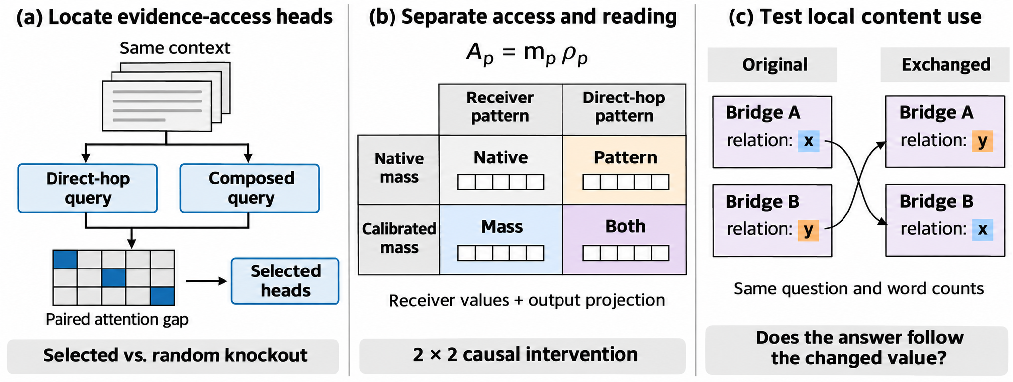
\includegraphics[width=\textwidth]{figures/figure2_diagnosis.pdf}
  \caption{\textbf{Overview of the mechanistic analysis.} (a) Direct second-hop and composed questions share evidence; their attention difference ranks heads, which are validated by knockout. (b) The four-arm intervention crosses paragraph mass and within-paragraph attention pattern, using receiver-computed values and original output-projection weights. (c) Reciprocal value exchanges test the complete repaired procedure's sensitivity to local relation values.}
  \label{fig:causal_framework}
\end{figure*}

To investigate this problem, we construct \dataset, a paired contextual reasoning protocol derived from 2WikiMultiHopQA \citep{ho2020constructing}. Each composed question is accompanied by two constituent queries under the same original context. As illustrated in \cref{fig:causal_framework}, the direct second-hop query explicitly names the bridge, creating a controlled reference for identifying attention heads whose allocation to the bridge changes during composition. Our analysis reveals a striking discrepancy: although composition fails in approximately half of the cases with correct constituent answers, the bridge paragraph remains recoverable from attention features in many failures. A linear readout fitted on training examples recovers the bridge in 72.2--86.0\% of these cases.

This observation motivates a closer examination of the selected heads' use of the bridge paragraph. We decompose its attention contribution into the total paragraph mass and the conditional distribution over its tokens. A crossed intervention independently calibrates the former and transfers the latter from a direct second-hop query. The interaction between these interventions reveals that the effectiveness of the local reading pattern depends on the access allocated to the paragraph. In Llama, for example, transferring the direct-query pattern changes accuracy by $-4$ points under native access but by $+12$ points after calibration. This functional dependence provides a concrete explanation of how a recoverable bridge address can coexist with ineffective use of the associated evidence.

Guided by this diagnosis, we introduce \method\ (\cref{fig:framework}), which couples selected-head adaptation with attention-guided evidence selection. Our contributions are threefold:
\begin{itemize}[leftmargin=*,itemsep=2pt,topsep=3pt,parsep=0pt]
\item \textbf{Methodology:} We develop a paired-query protocol and crossed attention interventions to separate access to relevant evidence from its conditional reading.
\item \textbf{Mechanism:} We show that bridge addresses remain recoverable during composition failures and that paragraph access determines the utility of direct-query reading patterns.
\item \textbf{Application:} We propose \method, improving composed accuracy by 33.3--39.9 percentage points with fewer than 1\% trainable model parameters. Matched ranking comparisons and reciprocal fact exchanges verify the role of evidence selection and local content.
\end{itemize}
